\documentclass{extarticle}
\usepackage[left=2cm,right=1.5cm,top=1.5cm, bottom=1.5cm]{geometry}

\usepackage{multirow}
\usepackage{hyperref}
\usepackage{url}

\usepackage{graphicx}
\usepackage{wrapfig}

\usepackage[utf8]{inputenc}
\usepackage[T1]{fontenc}
\usepackage[english, russian]{babel}


\begin{document}

\begin{titlepage}
	\begin{center}
		
		
		\textsc{\textbf{пояснительная записка \\
				к выпускной квалификационной работе на тему}}\\[2cm]
		
		% Title
		\textsc{Исследование влияния возможных систематических ошибок на результаты эксперимента по изучению временной инваринтности на ускорителе COSY \\[2.4cm] }
		
		
	\end{center}
	
	
	\begin{flushright}
		% Author and supervisor
		\begin{tabular}{rr}
			Студент-дипломник \underline{\hspace*{3cm}} & А.Е. Аксентьев \\
			&	группа А12-06 \\					
			Научный руководитель: Dr. rer. nat. \underline{\hspace*{3cm}} & Ю.В. Вальдау \\
			Консультант:          Доц., к.ф.-м.н. \underline{\hspace*{3cm}} & С.М. Полозов 	\\
			Рецензент:			  Доц., к.ф-м.н. \underline{\hspace*{3cm}} & А.А. Тищенко \\
			Зав. кафедрой:		  Проф., д.ф.-м.н. \underline{\hspace*{3cm}} & А.Н. Диденко
		\end{tabular}
		
	\end{flushright}
	
	\vfill
	
	
	\begin{center}
		\the\year{}
	\end{center}
	
	
	
\end{titlepage}

\tableofcontents
\pagebreak

\section*{Введение}
JEDI-коллаборация (J\"ulich Electric Dipole Moment Investigations) была создана в 2011 году с целью провести долгосрочный проект по измерению электрического дипольного момента (ЭДМ) заряженных частиц в накопительном кольце. На текущий момент, коллаборация базируется на синхротроне COSY (Institut f\"ur Kernphysik, Forschungszentrum J\"ulich, Юлих, Германия), где разрабатывает концептуальный дизайн накопительного кольца для поиска дейтронного ЭДМ.

\begin{wrapfigure}{R}{.5\textwidth}
	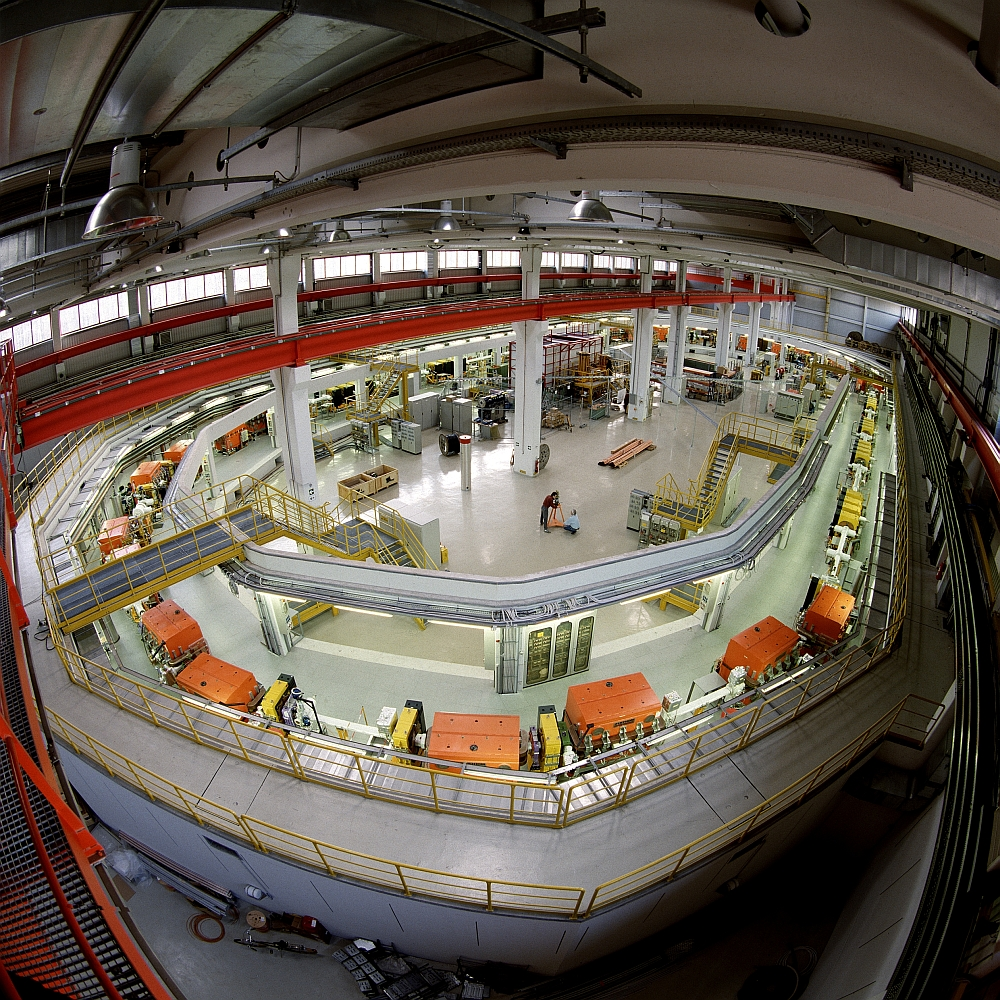
\includegraphics{img/cosy_220}
	\caption{COler SYnchrotron COSY в Исследовательском центре ``Юлих.''}
\end{wrapfigure}

Зачем искать ЭДМ.
	\begin{itemize}
		\item Барионная асимметрия вселенной;
		\item Условия Сахарова;
		\item Связь ЭДМ с нарушениями P-,T-симметрий
		\item Предсказания Стандартной Модели о величине ЭДМ;
		\item Если действительно найдём ЭДМ больше, чем предсказывает СМ, то значит нашли физику за её пределами.
	\end{itemize}
Поиск ЭДМ --- это мегазадача, над которой работает множество исселдовательских групп по всему миру. В частности, в JEDI коллаборации участвуют, среди прочих, исследователи из: CERN, Петербургского Института Ядерной Физики (Гатчина, Россия), Brookhaven National Laboratory (Аптон, Нью-Йорк, США), IKP Forschungszentrum J\"ulich (Юлих, Германия), LPSC (Гренобль Франция), Istituto Nazionale di Fisica Nucleare (Феррара, Италия).~\cite{JEDI}

\section{Финансирование}
В 2010 году директор Института Ядерной Физики (IKP) Исследовательского центра ``Юлих,'' профессор Ганс Штрёер получил грант от Европейского совета по научным исследованиям (European Research Council) на исследование возможности поляризации антипротонов.~\cite{ERCGrant10} Эти деньги были использованы на COSY для разработки и подтверждения работоспособности метода поляризации на протонах, чтобы в дальнейшем перенести эту методологию в CERN, на эксперименты с антипротонами.

В начале 2016 года, ERC выдал грант на пять лет (начиная с октября 2016) Юлихской группе (в лице доктора Штрёера), для дальнейших исследований в области Барионной Асимметрии вселенной.~\cite{ERCGrant16} Этот грант будет поддерживать также группы из Рейнско-Вестфальского Технического Университета Аахена (RWTH Aachen) в Германии, и Университета Феррары в Италии. Грант составляет 2.4 миллиарда евро.

\section{Логистика, организация, список заданий~\cite{ERCGrant12}}

Стоящие перед коллаборацией задачи можно разделить по следующим группам:
\begin{itemize}
	\item Организация:
		\begin{enumerate}
			\item Управление;
		\end{enumerate}
	\item Первые прямые наблюдения протонного и дейтронного ЭДМ на COSY:
		\begin{enumerate}
			\item Изучение времени когеренции спина на COSY;
			\item Прямые наблюдения протонного и дейтронного ЭДМ с использованием RF-E флиппера;
		\end{enumerate}
	\item Поляриметрия:
		\begin{enumerate}
			\item Разработка поляриметра; 
		\end{enumerate}
	\item Трэкинг спина:
		\begin{enumerate}
			\item Разработка программ-трекеров спина на основе пакета программ COSY Infinity; бенчмаркинг;
		\end{enumerate}
	\item Систематические ошибки:
		\begin{enumerate}
			\item Изучение систематических ошибок;
		\end{enumerate}
	\item Техническая разработка:
		\begin{enumerate}
			\item Разработка системы RF-E флиппера;
			\item Разработка детекторов позиции пучка;
		\end{enumerate}
	\item Теория:
		\begin{enumerate}
			\item Теоретические исследования.
		\end{enumerate}
\end{itemize}

\paragraph{Управление}
Управляющий совет состоит из 

Исполнительный совет коллаборации состоит из: Hans Str\"oher (председатель, директор IKP-2); Andreas Lerach, J\"org Pretz, Frank Rathmann (публичные представители); Volker Hejny (координатор по анализу данных); Alexander Nass (технический координатор). 

На сегодняшний день, коллаборация насчитывает 132 члена.

\section{Поиск ЭДМ в накопительном кольце}
Мегазадача требует мегаустановку, для своего решения. Как искать ЭДМ с помощью накопительного кольца.
	\begin{itemize}
		\item Что такое накопительное кольцо;
		\item Уравнение T-BMT;
		\item[\textbf{short:}] Условие заморозки спина => концепция Frozen Spin (BNL proposal~\cite{BNL});
		\item[\textbf{short:}] Незначительное ослабление полезного сигнала при релаксации FS условия => концепция Quasi-frozen Spin (Сеничев~\cite{Senichev});
		\item[\textbf{summary:}] Четыре фундаментальные концепции поиска ЭДМ в неидеальном накопительном кольце.
	\end{itemize}
	
\begin{figure}
	\centering
	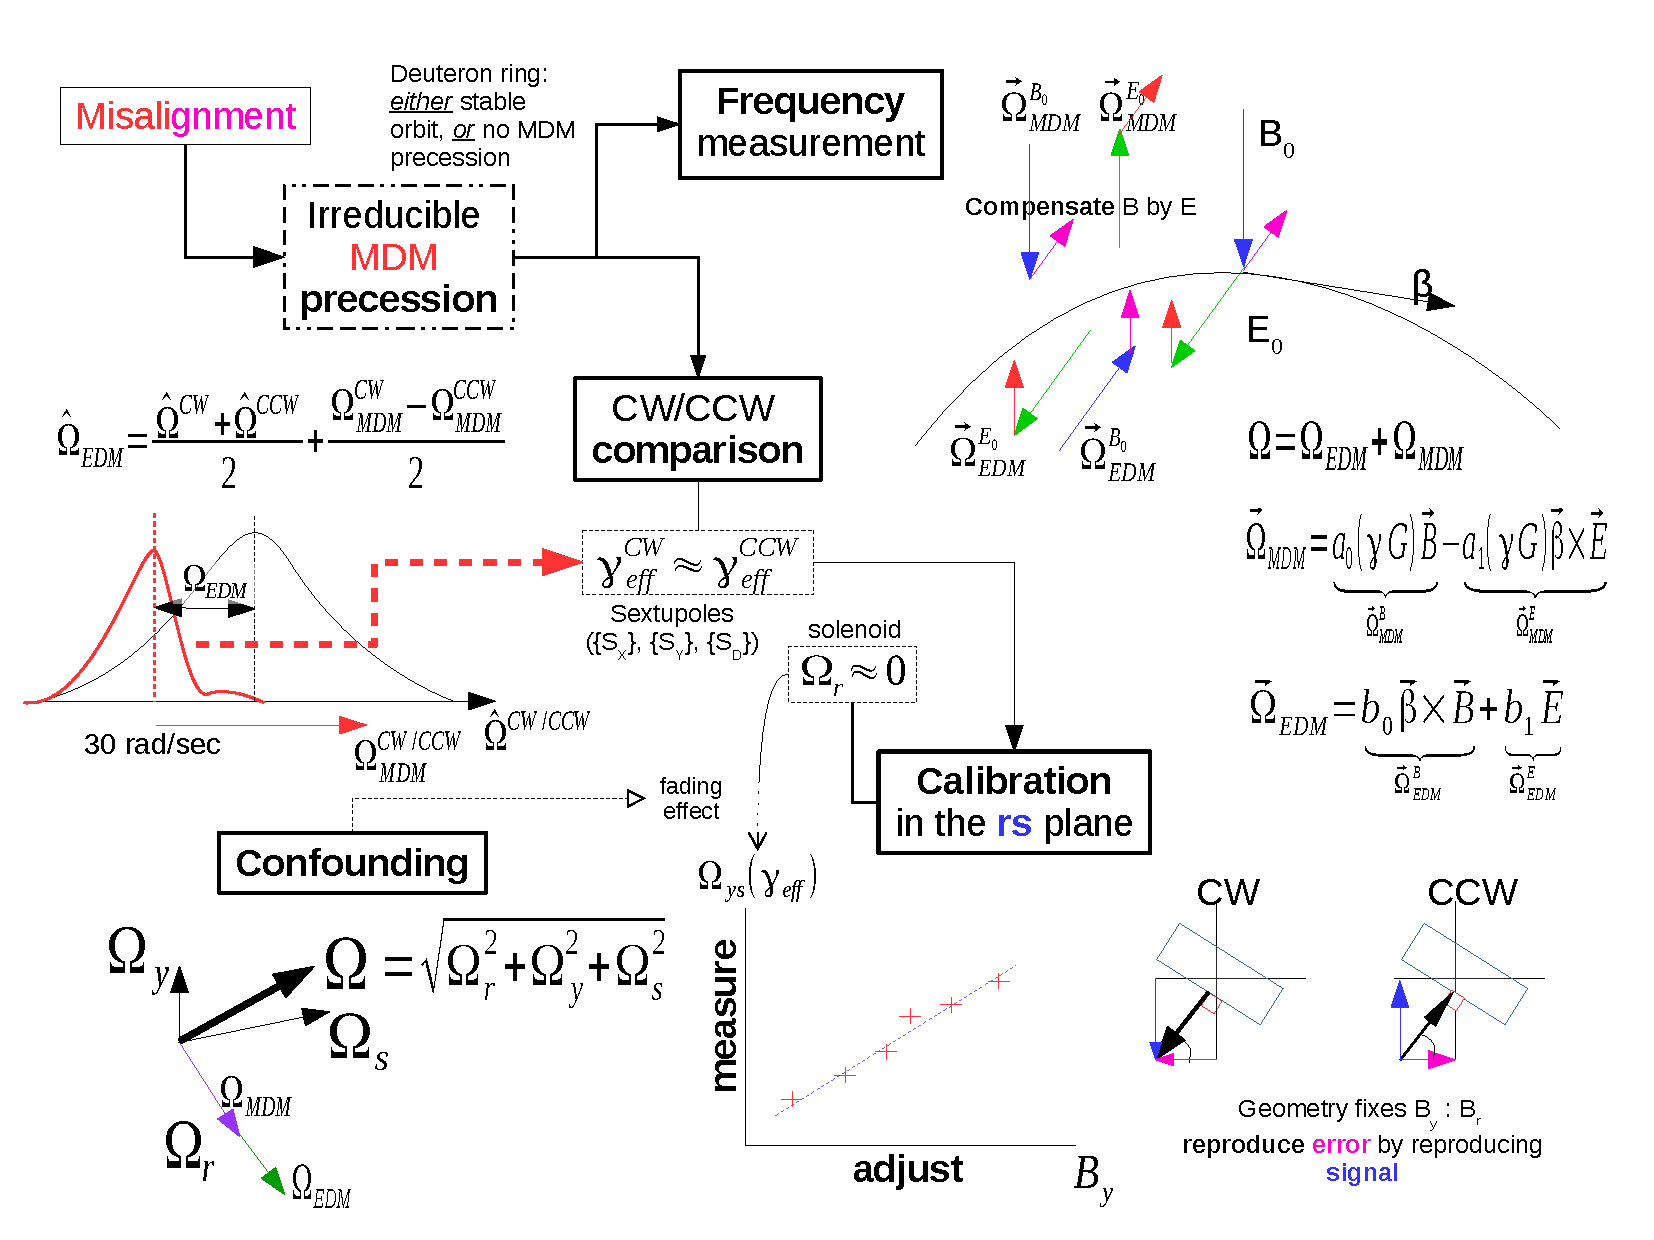
\includegraphics[scale=.6]{TheFourConcepts.pdf}
	\caption{Четыре концепции.}
\end{figure}

\section{Накопительные кольца для поиска дейтронного ЭДМ}
\subsection{FS кольцо}
	\subsubsection{Концепция эксперимента}
		Измеряем рост вертикальной компоненты поляризации за 1000 секунд.
	\subsubsection{Структура ускорителя}
	\subsubsection{Декогеренция спина}
		Ограничивает врямя измерения => нужно достичь 1000 секунд. Методы борьбы.
	\subsubsection{Систематические ошибки}
\subsection{QFS кольцо}
	\subsubsection{Концепция эксперимента}
		Фитируем сигнал, оцениваем частоту.
	\subsubsection{Структура ускорителя}
		Два варианта структуры.
	\subsubsection{Калибровка}
		Не подавляем МДМ прецессию спина => сравнение CW/CCW частот => калибровка. Как производится калибровка магнитного поля.
		
\section*{Заключение}
На данный момент, в исследовательской программе CERN планируется пауза на десять лет [в связи с анализом данных по Хиггсу?]. В связи с этим рассматривается список задач фундаментальной физики, которыми можно было бы заняться в это время. Среди приоритетных задач этого списка --- поиск ЭДМ. 

Поскольку протонное кольцо можно сделать полностью электростатическим (позволяет величина $G$), в то время как дейтронное принципиально требует магнитные элементы, если ЦЕРН решит заняться поиском ЭДМ, вероятнее всего будет построено протонное кольцо.
\begin{thebibliography}{0}
	\bibitem{JEDIatJuelich}
	Institute for Nuclear Physics, IKP-2: Experimental Hadron Dynamics. \url{http://www.fz-juelich.de/ikp/ikp-2/EN/Forschung/JEDI/_node.html}
	\bibitem{ERCGrant10}
	Str\"oher, H. Пресс-конференция. \url{https://www.fz-juelich.de/SharedDocs/Videos/PORTAL/EN/erc/erc-grant-stroeher.html}
	\bibitem{ERCGrant16}
	Lenisa, P., Pretz, J., Str\"oher, H. (2016). Storage ring steps up search for electric dipole moments. \textit{CERN Courier}. \url{http://cerncourier.com/cws/article/cern/65816}
	\bibitem{ERCGrant12}
	Rathmann, F. Application for an ERC Advanced Grant 2012. \url{http://collaborations.fz-juelich.de/ikp/jedi/public_files/proposals/merged_document.pdf}
	\bibitem{ERCGrant15}
	Str\"oher, H., Search for Electric Dipole Moments using Storage Rings, Horizon 2020 proposal, Excellence Science Call: ERC-2015-AdG. \url{http://collaborations.fz-juelich.de/ikp/jedi/public_files/proposals/Proposal-SEP-210276270.pdf}
	\bibitem{JEDI}
	JEDI Collaboration. \url{http://collaborations.fz-juelich.de/ikp/jedi/index.shtml}
	\bibitem{BNL}
	D. Anastassopoulos, V. Anastassopoulos, D. Babusci. AGS Proposal: Search for a permanent electric dipole moment of the deuteron nucleus at the $10^{-29} e\cdot cm$ level. [Internet]. BNL; 2008 [cited 2016 Nov 25]. Available from: \url{https://www.bnl.gov/edm/files/pdf/deuteron_proposal_080423_final.pdf}
	\bibitem{Senichev}
	Yurij Senichev. Search for the Charged Particle Electric Dipole Moments in Storage Rings. In: 25th Russian Particle Accelerator Conf(RuPAC’16), St Petersburg, Russia, November 21-25, 2016 [Internet]. JACOW, Geneva, Switzerland; 2017 [cited 2017 Apr 5]. p. 6–10. Available from: \url{http://accelconf.web.cern.ch/AccelConf/rupac2016/papers/mozmh03.pdf}
	
\end{thebibliography}
\end{document}